\documentclass[11pt]{amsart}
\usepackage[top=2.5 cm, bottom=2.5 cm, left=1.05in, right=1.05in]{geometry}
%\geometry{a4paper} % or letter or a5paper or ... etc
% \geometry{landscape} % rotated page geometry
\usepackage[applemac]{inputenc}
\usepackage{amsmath,amssymb} 
% See the ``Article customise'' template for come common customisations
\usepackage{hyperref}
\usepackage{amsmath}
\usepackage{lineno}
\usepackage{graphicx}
\usepackage{color}
\title{Viola-Jones faces recognition}
\author{Alessandro Manzotti}
%\date{} % delete this line to display the current date

%%% BEGIN DOCUMENT
\begin{document}

\maketitle
%\tableofcontents

In this homework, we consider the problem of face detection. That is, given an image, we wish to identify and locate instances of a general object class, i.e. faces within the image. A complete object detection system consists of a sliding window and a classifier. As the sliding window scans the image, the classifier makes a decision regarding whether or not the portion of the image occupied by the sliding window is an instance of a particular class or not. Obviously, such a classifier must have a very low false positive rate as the number of negative samples will drastically outnumber the positive samples.
We implement an Adaboost classifier with Haar-like features. Such a classifier consists of a weighted sum of many weak classifiers. To obtain a sufficiently low false positive rate, we cascade several Adaboost classifiers, where at each stage of the cascade only the samples classified as positive are allowed to pass through. Thus, increasingly difficult false positives are pruned away at each stage.

\section{Haar-like features}

The training images considered in this homework are of size $64\times64$ pixels.
From these image, we extract a subset of Haar-like features, which are computed using vertical and horizontal differencing operators. The features are computed efficiently exploiting the integral image.
Given the computational power and time I decided to use just the simple rectangular Haar feature starting with a minimum size of 6 pixels (3+3 pixels). I use a stride of size 4 in the final run. In total I have used a subset of \textbf{61440 features}.
\begin{figure}[htbp]
\begin{center}
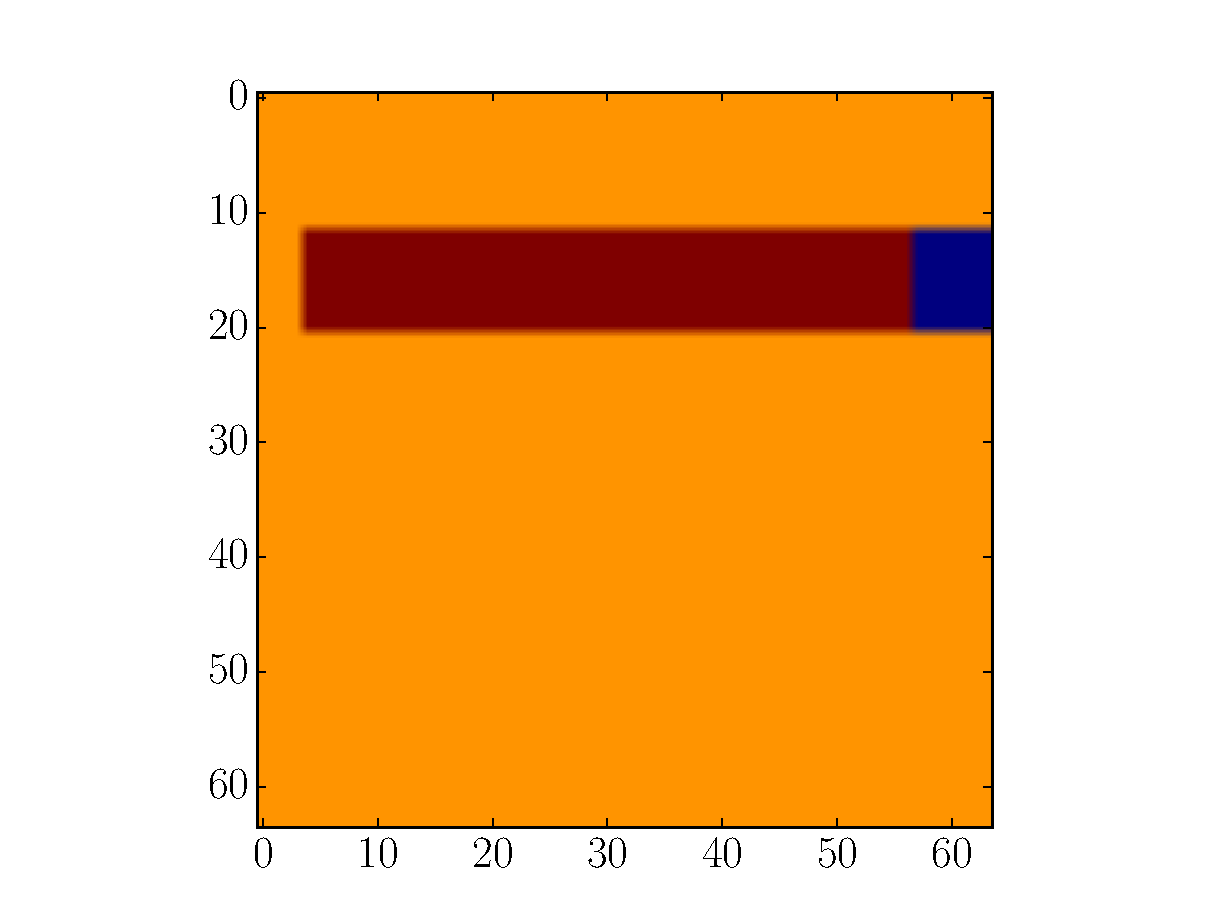
\includegraphics[scale=0.2]{feature3.pdf}
\caption{An example of an important feature (weak classifier for AdaBoost) for face-classification.}
\label{default}
\end{center}
\end{figure}



\section{Single AdaBoost}

As suggested I have used a simple AdaBoost. The final classifier threshold was set to avoid any false negative (depending on the stage it was $1.3<\Theta<3.2$). An example of one of the best weak classifier and the train error for a single AdaBoost are shown in Fig. 1-2-3.

\begin{figure}[htbp]
\begin{center}
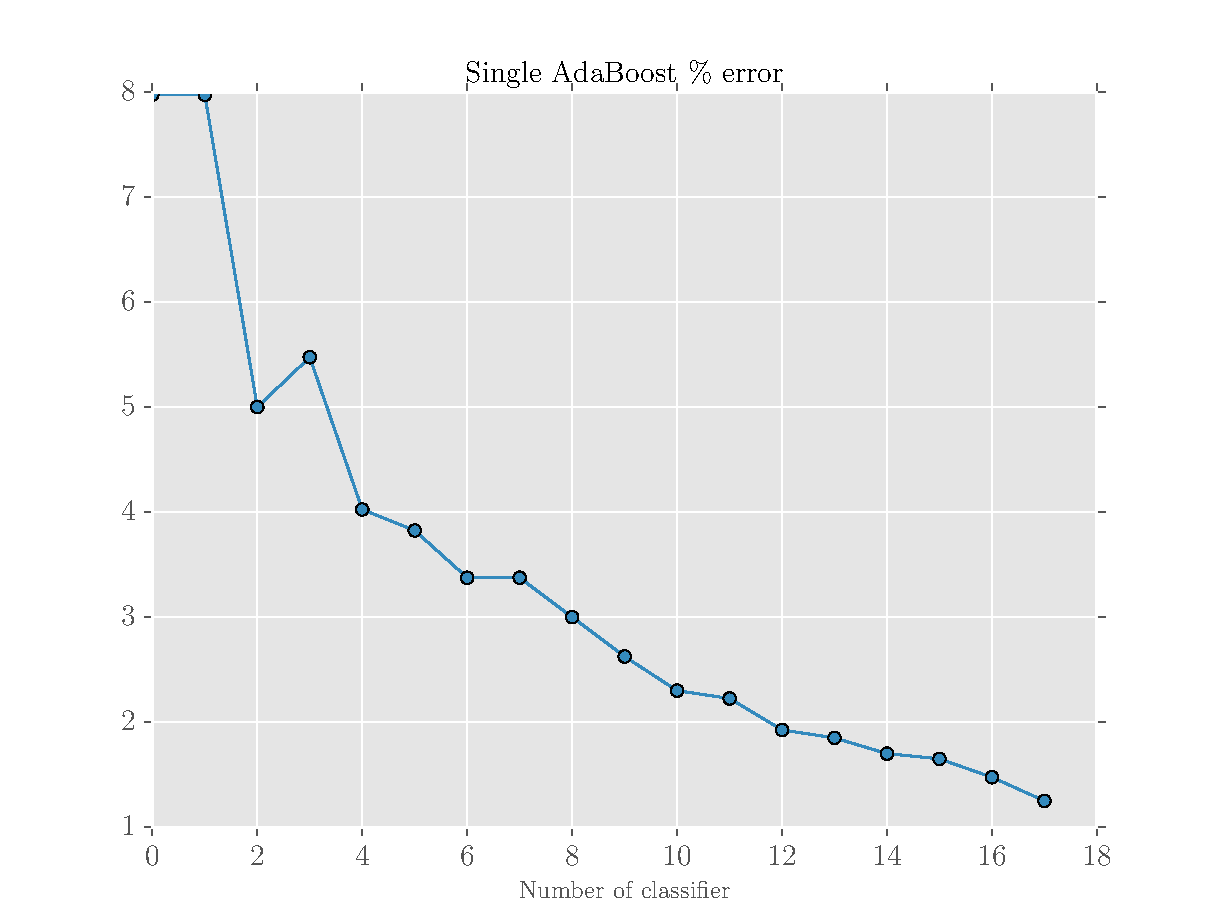
\includegraphics[scale=0.5]{single_ada.pdf}
\caption{Training error for a single AdaBoost as a function of the number of ``weak lerner'' used.}
\label{default}
\end{center}
\end{figure}

\begin{figure}[htbp]
\begin{center}
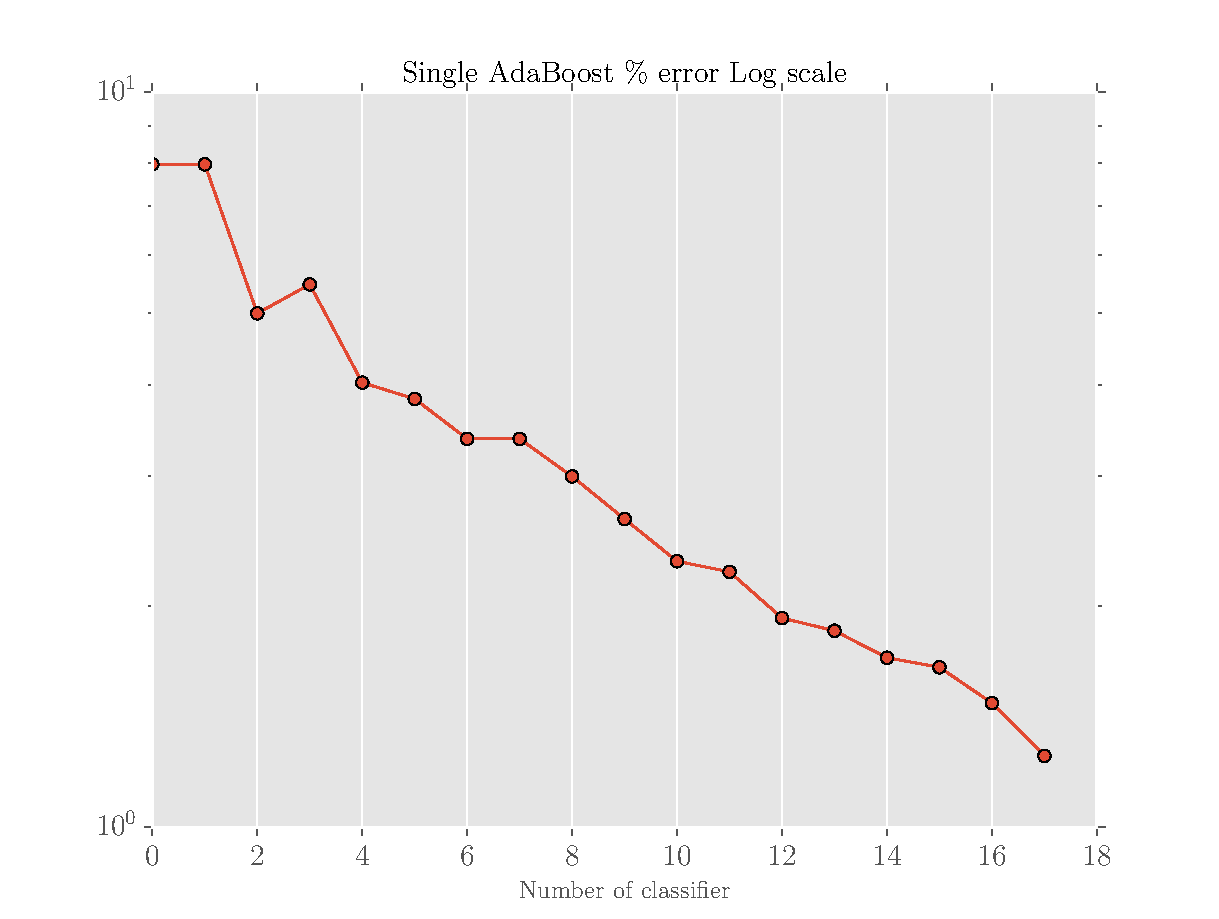
\includegraphics[scale=0.5]{single_ada_log.pdf}
\caption{LOG SCALE. Training error for a single AdaBoost as a function of the number of ``weak lerner'' used. As can be seen and as expected the error decrease exponetially.}
\label{default}
\end{center}
\end{figure}

\begin{figure}[htbp]
\begin{center}
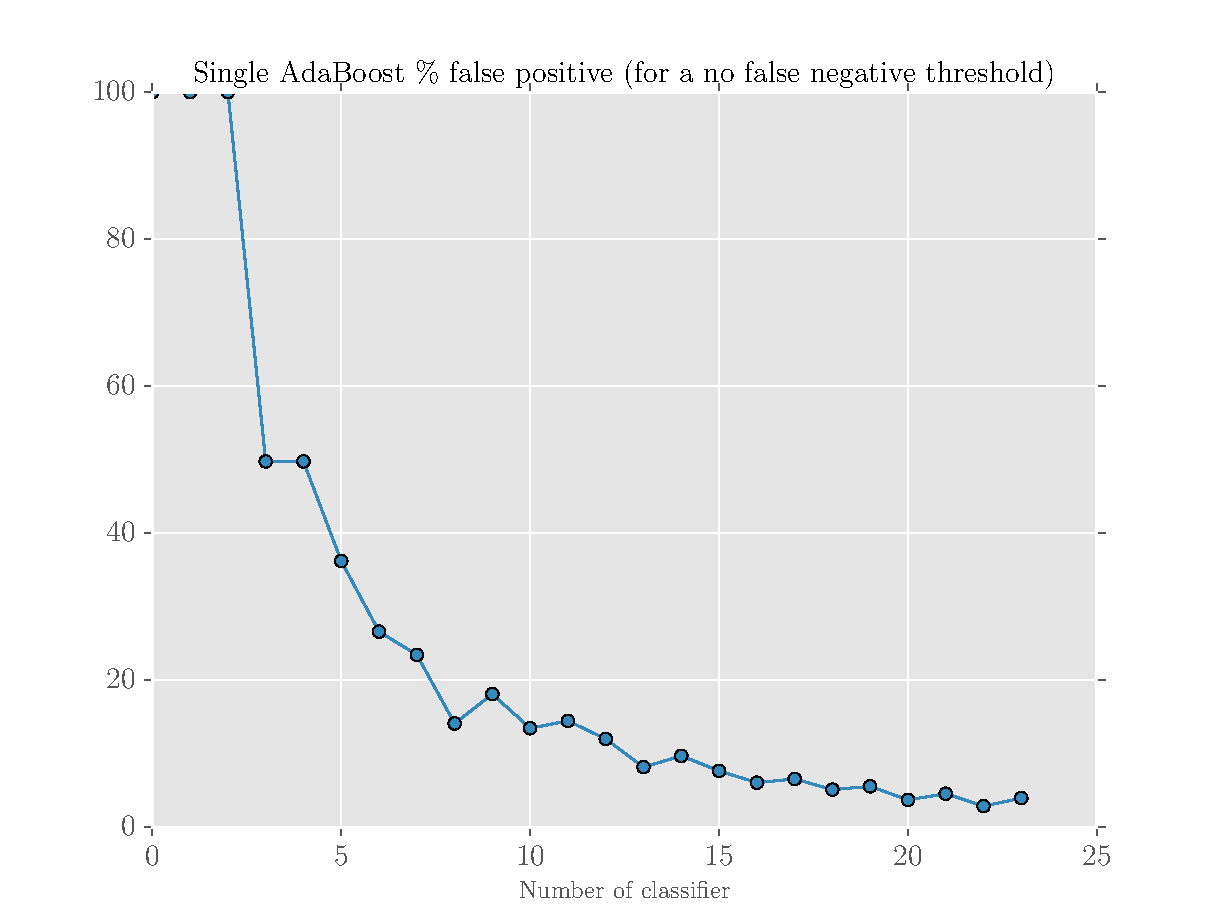
\includegraphics[scale=0.5]{single_ada_false_pos2.pdf}
\caption{This shows the number of false positive for a single AdaBoost (no cascade) as a function of the number of ``weak lerner'', Haar features in this case, used in the classification. In this case a threshold was set so that there were no false negative. With 5 features we can push the error to $~18\%$. Using a cascade of classifier we can achieve a fairly low rate of false positive.}
\label{default}
\end{center}
\end{figure}



\section{Cascade}
Being computationally limited we fixed the final cascade number to 6 AdaBoost classifiers.
Training time and errors are showed in Table 1.
\begin{table}[htbp]
\caption{TRAINING THE CASCADE. These refers to 61440 features and no parallelization implemented in the Python code. The classifier threshold was set to avoid false negative.}\begin{center}
\begin{tabular}{|c|c|c|}
\hline
Stage & Training time (s)& Error \\
\hline
1&220&10\%\\ 
\hline
2&390&8\%\\ 
\hline
3&390&6\%\\ 
\hline
4&421&3.7\%\\ 
\hline
5&513&2.8\%\\ 
\hline
6&636&2.5\%\\ 
\hline
\end{tabular}
\end{center}
\end{table}%


\section{Evaluate on images}
I just use a sliding window on the test image. To save time I did not check all the possible patches but I move the sliding window for 8 pixels at each move (either vertical or horizontal). This still takes a lot of time and a parallelization of the feature computation and patch evaluation would probably be needed for this.


\section{Overlapping and plot}
I noticed that most faces are detected at multiple nearby positions, while false detections often occur with less consistency. I tried to use this observation to eliminate some false detections. For each location at which a face is detected, the number of detections within a specified neighborhood of that location can be counted. If the number is above a threshold, then that location is classified as a face. For this reason I applied a Gaussian filter to the 
binary matrix (1 face 0 non face). After that I applied a threshold to retain only a small percentage. The goal of this was to reduce the overlapping while excluding very isolated, and for this reason likely false, positive detection.

After that I finally reduce the overlapping with a simple non-maximum suppression edge thinning technique. Basically I computed the area overlapping of all the squared 64x64 detection patches and discard all of those that overlaps for more than a threshold value.


%%
%%The centroid of the nearby detections defines the location of the detection result, thereby collapsing multiple detections. In the experiments section, this heuristic will be referred to as ``thresholding''.
%
%
%
%The implementation of these two heuristics is illustrated in Figure 6. Each detection by the network at a particular location and scale is marked in an image pyramid, labelled the ``output'' pyramid. Then, each location in the pyramid is replaced by the number of detections in a specified neighborhood of that location. This has the effect of ``spreading out'' the detections. Normally, the neighborhood extends an equal number of pixels in the dimensions of scale and position, but for clarity in Figure 6 detections are only spread out in position. A threshold is applied to these values, and the centroids (in both position and scale) of all above threshold regions are computed. All detections contributing to the centroids are collapsed down to single points. Each centroid is then examined in order, starting from the ones which had the highest number of detections within the specified neighborhood. If any other centroid locations represent a face overlapping with the current centroid, they are removed from the output pyramid. All remaining centroid locations constitute the final detection result.

\section{Results}

The final results is shown in Fig.5. 
Given the fact that I have used given time and computational power, not many and very simple Haar features, the classifier picks all the patches with a significant dynamic contrast.
This means not only faces but also hands and patterns in people dresses. Significant is the example of the girl in the lower-right corner. Overall however a fair number of faces has been detected.

\begin{figure}[htbp]
\begin{center}
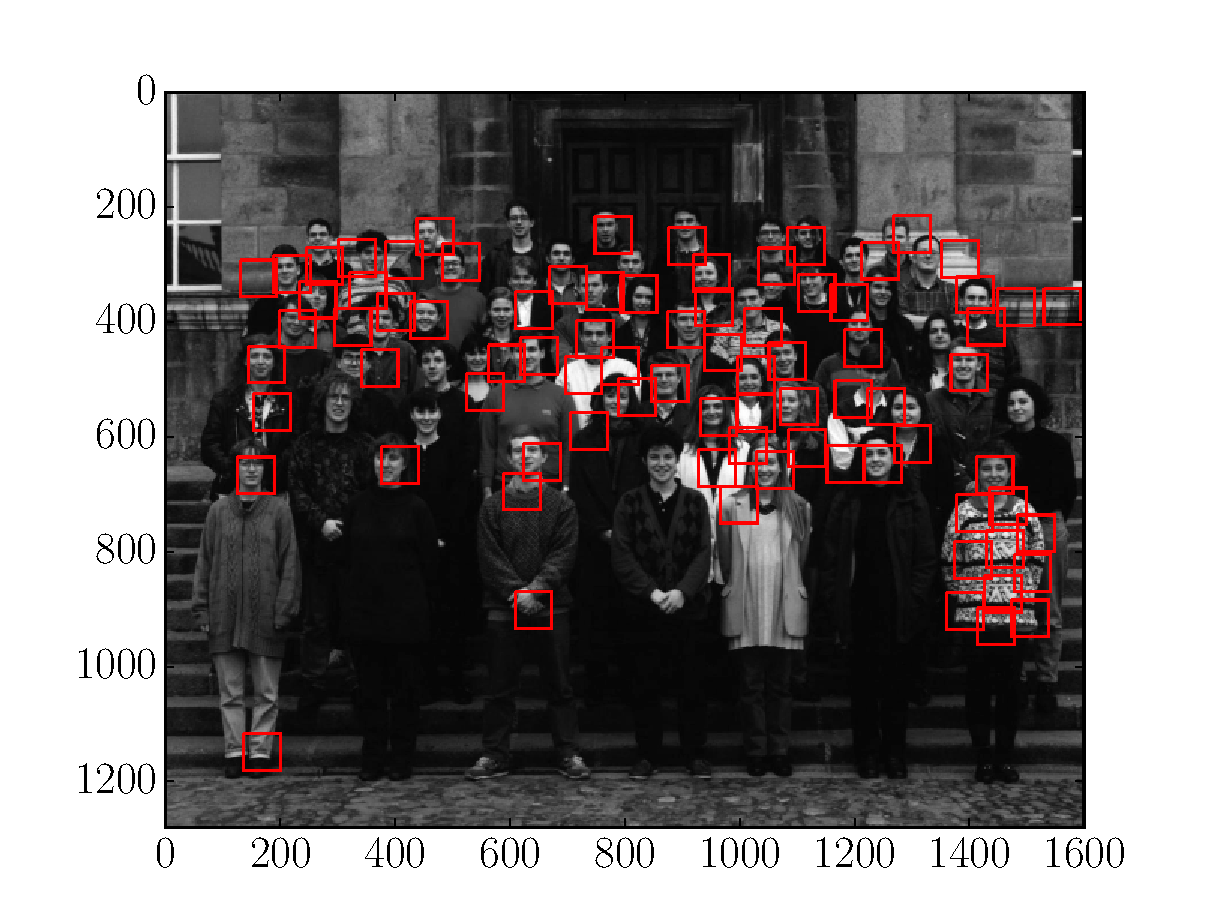
\includegraphics[scale=0.5]{final.pdf}
\caption{}
\label{default}
\end{center}
\end{figure}

\section{Possible improvements}
\begin{itemize}
\item More Haar features. To implement that, a simple parallel code might be needed. Most of the training and evaluation can be embarassily parallelizwd among the 4000 images (training) or patches (evaluation). This would have probably allowed me to use more features, while keeping the code in a reasonable time frame. The main issues however was the size of the features. I tried to save them as float16 but still it was a significant challenge for my laptop.

\item Embarassing parallelism.
\item Use margins. Indeed one can use the last Adaboost classifier of the cascade to give also an estimate of the significance of each detection. Notice that this margin, $|\sum^{T}_{t=1}\alpha_{t}h_{t}(x)|$, is what AdaBoost tends to maximize. This information can be passed to the gaussian filter (for example not using a binary matrix detected-not detected but a matrix of the significance of the detection) and the overlapping filter to make a more informed guess.
\end{itemize}








\end{document}